% ════════════════════════════════════════════
% 4. 回归模型与预测能力
% ════════════════════════════════════════════
\section{回归模型与预测能力（对应 2.3）}

\subsection{模型设定与候选比较（对应 2.3.1）}

\begin{center}
\begin{minipage}{\textwidth}
\noindent\rule{\textwidth}{0.9pt}\par\nobreak\vspace{2pt}
\refstepcounter{algocnt}\noindent\textbf{算法 \thealgocnt\quad 曝光回归的建模、选择与效应测算流程}\label{alg:pipeline}\par\nobreak\vspace{2pt}
\noindent\rule{\textwidth}{0.4pt}\par\nobreak\vspace{4pt}
{\small
\noindent\textbf{输入：}清洗数据 $\mathcal{D}$（$n=500$、$p=8$）；候选设定 $\mathcal{M}=\{M_0,\dots,M_4\}$；折数 $K=10$；模拟次数 $B=1000$。\par\vspace{2pt}
\noindent\textbf{输出：}$M^{*}$；系数与 95\% 置信区间；付费与类型效应；组内联合检验 $p$。\par\vspace{4pt}
\noindent{\color{gray}// 阶段 1：编码与共线判别}\par
\hangindent=1.6em\hangafter=1 \hspace*{1.2em}1\ \ $X\leftarrow$ 独热编码 $(X_2,X_3,X_4,X_5,\text{时段})$，$y\leftarrow\log(1+Y_1)$；若 $\max\mathrm{VIF}>10$ 且 $|\rho(\log X_1,X_4)|\ge0.9$ 且月内方差占比 $<5\%$，则从 $\mathcal{M}$ 删去 $\log X_1$ 与月份并列的设定。\par\vspace{3pt}
\noindent{\color{gray}// 阶段 2：主循环（复杂度 $O(Knp^2)$）}\par
\hangindent=1.6em\hangafter=1 \hspace*{1.2em}2\ \ \textbf{for each} $M_j\in\mathcal{M}$ \textbf{do} $(\hat\beta_j,\widehat{\mathrm{Cov}}_j)\leftarrow\mathrm{fitHC3}(y,X_{M_j})$；$(R^2_j,\mathrm{CV}R^2_j)\leftarrow\mathrm{kfoldCV}(y,X_{M_j},K)$。\par\vspace{3pt}
\noindent{\color{gray}// 阶段 3：终止条件——交叉验证最优且参数最少}\par
\hangindent=1.6em\hangafter=1 \hspace*{1.2em}3\ \ $M^{*}\leftarrow\arg\max_{j}\mathrm{CV}R^2_j$，并列时取参数个数最小者。\par\vspace{3pt}
\noindent{\color{gray}// 阶段 4：诊断与效应测算}\par
\hangindent=1.6em\hangafter=1 \hspace*{1.2em}4\ \ 执行 BP / JB / Cook 检验，异方差时沿用 HC3；$s\leftarrow\mathrm{duanSmearing}(\hat\beta^{*})$；$(\hat\tau,\text{CI})\leftarrow\mathrm{simulateCI}(\hat\beta^{*},\widehat{\mathrm{Cov}}^{*},B,s)$；对类型、主题、时段子样本重估 $M^{*}$，得组内联合 Wald $p$。\par\vspace{3pt}
\hangindent=1.6em\hangafter=1 \hspace*{1.2em}5\ \ \textbf{return} $M^{*},\hat\beta^{*},\hat\tau,\text{CI}$。\par}
\vspace{2pt}\noindent\rule{\textwidth}{0.9pt}\par\vspace{6pt}
\end{minipage}
\end{center}

因变量取 $\log(1+Y_1)$，解释变量为发帖决策变量与时间控制项，估计方法为普通最小二乘、推断采用 HC3 稳健标准误。设定从“全模型”出发逐步剔除不可识别或冗余的项，形成五个候选：M0 为均值基线，M1 为含粉丝规模与月份的全模型，M2 去掉粉丝规模、保留月份固定效应，M3 只留粉丝规模，M4 用线性月份替代月份哑变量。五个候选的拟合与十折交叉验证结果见表\ref{tab:cv}：M2 的交叉验证 $R^2$ 最高（0.101）、CV RMSE 最低（1.101），样本内 $R^2=0.207$、调整 $R^2=0.165$；M1 多一个参数而交叉验证表现反而略差，说明粉丝规模提供的是与月份重复的信息。M0 的交叉验证 $R^2$ 为 $-0.021$，均值基线不具备预测能力。

{\small
\begin{longtable}{>{\centering\arraybackslash}p{0.080\textwidth}>{\centering\arraybackslash}p{0.100\textwidth}>{\centering\arraybackslash}p{0.090\textwidth}>{\centering\arraybackslash}p{0.105\textwidth}>{\centering\arraybackslash}p{0.100\textwidth}>{\centering\arraybackslash}p{0.115\textwidth}>{\centering\arraybackslash}p{0.100\textwidth}>{\centering\arraybackslash}p{0.115\textwidth}>{\centering\arraybackslash}p{0.115\textwidth}}
  \caption{五个候选模型的拟合、整体显著性与十折交叉验证}
  \label{tab:cv} \\
  \toprule
  模型 & 参数个数 & $R^2$ & 调整 $R^2$ & 整体 $F$ & $F$ 检验 $p$ & CV $R^2$ & CV RMSE & CV MAE \\
  \midrule
  \endfirsthead
  \caption{五个候选模型的拟合、整体显著性与十折交叉验证（续）} \\
  \toprule
  模型 & 参数个数 & $R^2$ & 调整 $R^2$ & 整体 $F$ & $F$ 检验 $p$ & CV $R^2$ & CV RMSE & CV MAE \\
  \midrule
  \endhead
  \bottomrule
  \endfoot
  M0 & 1 & 0 & 0 & — & — & -0.0212 & 1.1753 & 0.9133 \\
  M1 & 27 & 0.2069 & 0.1633 & 4.7465 & $<$0.001 & 0.0972 & 1.1031 & 0.8351 \\
  M2 & 26 & 0.2068 & 0.1650 & 4.9443 & $<$0.001 & 0.1010 & 1.1007 & 0.8328 \\
  M3 & 16 & 0.1606 & 0.1346 & 6.1756 & $<$0.001 & 0.0935 & 1.1065 & 0.8220 \\
  M4 & 17 & 0.1664 & 0.1388 & 6.0265 & $<$0.001 & 0.0972 & 1.1042 & 0.8215 \\
\end{longtable}
}



建模、选择与效应测算的整体流程见算法\ref{alg:pipeline}。算法的关键设计是把“共线判别”放在模型拟合之前，避免先拟合再删变量的循环论证；终止条件不是样本内拟合最好，而是交叉验证 $R^2$ 最大且参数个数最少。



\subsection{估计结果（对应 2.3.1）}

最终模型 M2 的系数见表\ref{tab:coef}，该模型 $R^2=0.207$、调整 $R^2=0.165$，整体 $F=4.94$（$p<0.001$），即 26 个参数联合显著。控制月份、星期、时段后，付费帖子的 $\log(1+Y_1)$ 比自然帖子高 0.337（HC3 标准误 0.120，$p=0.005$）；类型维度上，Status 与 Video 分别比 Photo 高 1.154 与 1.590，Link 与 Photo 无显著差异（$p=0.643$）；主题 2 与主题 3 分别比主题 1 低 0.478 与 0.315，前者 $p<0.001$、后者 $p=0.019$；凌晨与下午晚间相对上午不显著（$p=0.150$、$p=0.638$），星期各水平同样不显著。模型常数项 9.247 对应基准组合（Photo、主题 1、1 月、周一、上午、自然帖）的期望对数曝光。图\ref{fig:forest}把主效应点估计与 95\% 置信区间并排呈现，显著为正、显著为负与不显著三档分别用深蓝、红与灰区分。

\needspace{30\baselineskip}
{\small
\begin{longtable}{>{\centering\arraybackslash}p{0.240\textwidth}>{\centering\arraybackslash}p{0.100\textwidth}>{\centering\arraybackslash}p{0.100\textwidth}>{\centering\arraybackslash}p{0.080\textwidth}>{\centering\arraybackslash}p{0.120\textwidth}>{\centering\arraybackslash}p{0.120\textwidth}>{\centering\arraybackslash}p{0.080\textwidth}>{\centering\arraybackslash}p{0.080\textwidth}}
  \caption{最终模型 M2 的系数估计}
  \label{tab:coef} \\
  \toprule
  变量 & 系数 & 标准误 & $p$ & CI 下限 & CI 上限 & VIF & 显著性 \\
  \midrule
  \endfirsthead
  \caption{最终模型 M2 的系数估计（续）} \\
  \toprule
  变量 & 系数 & 标准误 & $p$ & CI 下限 & CI 上限 & VIF & 显著性 \\
  \midrule
  \endhead
  \bottomrule
  \endfoot
  常数项 & 9.2468 & 0.2052 & $<$0.001 & 8.8436 & 9.65 & — & *** \\
  类型：Status & 1.1538 & 0.1235 & $<$0.001 & 0.9110 & 1.3966 & 1.2748 & *** \\
  类型：Link & 0.1215 & 0.2619 & 0.643 & -0.3930 & 0.6361 & 1.1356 &  \\
  类型：Video & 1.5896 & 0.4017 & $<$0.001 & 0.8003 & 2.3789 & 1.0626 & *** \\
  主题：2 & -0.4784 & 0.1352 & $<$0.001 & -0.7440 & -0.2128 & 1.7829 & *** \\
  主题：3 & -0.3147 & 0.1337 & 0.019 & -0.5775 & -0.0519 & 1.527 & * \\
  月份：2月 & 0.8765 & 0.3037 & 0.004 & 0.2798 & 1.4733 & 2.0388 & ** \\
  月份：3月 & -0.0414 & 0.3095 & 0.894 & -0.6495 & 0.5667 & 2.5431 &  \\
  月份：4月 & 0.3808 & 0.1768 & 0.032 & 0.0333 & 0.7283 & 2.835 & * \\
  月份：5月 & 0.1908 & 0.1710 & 0.265 & -0.1453 & 0.5269 & 2.362 &  \\
  月份：6月 & 0.1491 & 0.1850 & 0.421 & -0.2144 & 0.5125 & 2.82 &  \\
  月份：7月 & 0.3131 & 0.1900 & 0.100 & -0.0603 & 0.6866 & 2.9706 &  \\
  月份：8月 & 0.1120 & 0.2484 & 0.652 & -0.3762 & 0.6002 & 2.3062 &  \\
  月份：9月 & -0.1259 & 0.1877 & 0.503 & -0.4947 & 0.2429 & 2.4259 &  \\
  月份：10月 & -0.4711 & 0.2136 & 0.028 & -0.8909 & -0.0514 & 3.232 & * \\
  月份：11月 & 0.0355 & 0.1956 & 0.856 & -0.3489 & 0.4198 & 2.808 &  \\
  月份：12月 & -0.1012 & 0.1644 & 0.538 & -0.4242 & 0.2218 & 2.8513 &  \\
  星期：周二 & 0.0939 & 0.1977 & 0.635 & -0.2946 & 0.4823 & 1.7593 &  \\
  星期：周三 & -0.0191 & 0.1920 & 0.921 & -0.3963 & 0.3582 & 1.7682 &  \\
  星期：周四 & 0.2585 & 0.2084 & 0.215 & -0.1509 & 0.6679 & 1.847 &  \\
  星期：周五 & -0.0929 & 0.1770 & 0.600 & -0.4407 & 0.2548 & 1.7946 &  \\
  星期：周六 & -0.1607 & 0.1852 & 0.386 & -0.5246 & 0.2032 & 1.9324 &  \\
  星期：周日 & -0.2214 & 0.1753 & 0.207 & -0.5658 & 0.1231 & 1.8974 &  \\
  时段：凌晨 & 0.1643 & 0.1139 & 0.150 & -0.0595 & 0.3881 & 1.3177 &  \\
  时段：下午晚间 & 0.0751 & 0.1595 & 0.638 & -0.2383 & 0.3885 & 1.5198 &  \\
  付费（X7=1） & 0.3374 & 0.1195 & 0.005 & 0.1025 & 0.5723 & 1.0772 & ** \\
  \bottomrule
\end{longtable}
}
\vspace{-4pt}
{\footnotesize\raggedright 注：标准误为 HC3 稳健标准误；CI 为 95\% 置信区间；*** 为 $p<0.001$，** 为 $p<0.01$，* 为 $p<0.05$。\par}
\vspace{4pt}


\needspace{30\baselineskip}
{\small
\begin{longtable}{>{\centering\arraybackslash}p{0.240\textwidth}>{\centering\arraybackslash}p{0.100\textwidth}>{\centering\arraybackslash}p{0.100\textwidth}>{\centering\arraybackslash}p{0.080\textwidth}>{\centering\arraybackslash}p{0.120\textwidth}>{\centering\arraybackslash}p{0.120\textwidth}>{\centering\arraybackslash}p{0.080\textwidth}>{\centering\arraybackslash}p{0.080\textwidth}}
  \caption{全模型 M1 的系数估计（含粉丝规模与月份并列）}
  \label{tab:coef_m1} \\
  \toprule
  变量 & 系数 & 标准误 & $p$ & CI 下限 & CI 上限 & VIF & 显著性 \\
  \midrule
  \endfirsthead
  \caption{全模型 M1 的系数估计（含粉丝规模与月份并列）（续）} \\
  \toprule
  变量 & 系数 & 标准误 & $p$ & CI 下限 & CI 上限 & VIF & 显著性 \\
  \midrule
  \endhead
  \bottomrule
  \endfoot
  常数项 & -0.2487 & 43.3613 & 0.995 & -85.4533 & 84.9559 & — &  \\
  log(粉丝规模) & 0.8360 & 3.8193 & 0.827 & -6.6689 & 8.341 & 124.9 &  \\
  类型：Status & 1.1519 & 0.1244 & $<$0.001 & 0.9075 & 1.3963 & 1.2774 & *** \\
  类型：Link & 0.1223 & 0.2624 & 0.641 & -0.3934 & 0.6380 & 1.1358 &  \\
  类型：Video & 1.5881 & 0.4014 & $<$0.001 & 0.7993 & 2.3769 & 1.0629 & *** \\
  主题：2 & -0.4768 & 0.1356 & $<$0.001 & -0.7433 & -0.2104 & 1.7872 & *** \\
  主题：3 & -0.3132 & 0.1336 & 0.019 & -0.5757 & -0.0507 & 1.5311 & * \\
  月份：2月 & 0.8136 & 0.4183 & 0.052 & -0.0084 & 1.6357 & 3.7348 &  \\
  月份：3月 & -0.1740 & 0.6222 & 0.780 & -1.3965 & 1.0486 & 12.7489 &  \\
  月份：4月 & 0.1698 & 0.9862 & 0.863 & -1.7682 & 2.1077 & 37.6861 &  \\
  月份：5月 & -0.0772 & 1.2353 & 0.950 & -2.5046 & 2.3501 & 45.1579 &  \\
  月份：6月 & -0.1675 & 1.4654 & 0.909 & -3.047 & 2.712 & 79.8366 &  \\
  月份：7月 & -0.0344 & 1.6088 & 0.983 & -3.1958 & 3.1269 & 100.8 &  \\
  月份：8月 & -0.2543 & 1.6984 & 0.881 & -3.5916 & 3.0829 & 76.2541 &  \\
  月份：9月 & -0.5089 & 1.7744 & 0.774 & -3.9957 & 2.9778 & 87.661 &  \\
  月份：10月 & -0.8613 & 1.8108 & 0.634 & -4.4195 & 2.6969 & 143.0 &  \\
  月份：11月 & -0.3627 & 1.841 & 0.844 & -3.9802 & 3.2547 & 115.7 &  \\
  月份：12月 & -0.5064 & 1.8714 & 0.787 & -4.1837 & 3.171 & 131.3 &  \\
  星期：周二 & 0.0930 & 0.1980 & 0.639 & -0.2961 & 0.4822 & 1.76 &  \\
  星期：周三 & -0.0207 & 0.1927 & 0.915 & -0.3993 & 0.3580 & 1.7707 &  \\
  星期：周四 & 0.2593 & 0.2101 & 0.218 & -0.1535 & 0.6721 & 1.8477 &  \\
  星期：周五 & -0.0915 & 0.1778 & 0.607 & -0.4407 & 0.2578 & 1.7968 &  \\
  星期：周六 & -0.1604 & 0.1856 & 0.388 & -0.5251 & 0.2044 & 1.9325 &  \\
  星期：周日 & -0.2207 & 0.1758 & 0.210 & -0.5662 & 0.1249 & 1.898 &  \\
  时段：凌晨 & 0.1657 & 0.1135 & 0.145 & -0.0573 & 0.3886 & 1.3216 &  \\
  时段：下午晚间 & 0.0725 & 0.1623 & 0.655 & -0.2464 & 0.3913 & 1.5302 &  \\
  付费（X7=1） & 0.3371 & 0.1200 & 0.005 & 0.1012 & 0.5730 & 1.0774 & ** \\
  \bottomrule
\end{longtable}
}
\vspace{-4pt}
{\footnotesize\raggedright 注：标准误为 HC3 稳健标准误；CI 为 95\% 置信区间；M1 中 $\log X_1$ 的 VIF 为 124.9，月份组最大 143.0，系数不可识别。\par}
\vspace{4pt}


表\ref{tab:coef_m1}给出全模型 M1 的完整系数表（27 个参数）。它是题面要求的“真实系数表”的原始估计：$\log X_1$ 的系数 0.836（HC3 标准误 3.819、$p=0.827$）几乎没有信息量，常数项标准误达 43.36，根源是 $\log X_1$ 与月份哑变量并列后 VIF 达到 124.9；这正是第 3.3 节判定不可识别、并最终以 M2 作为解释模型的直接证据。两表对照可以看出：剔除 $\log X_1$ 后，付费、类型与主题的系数变动都在 0.01 以内，说明主效应并未因共线处理而改变。


\begin{figure}[htbp]
  \centering
  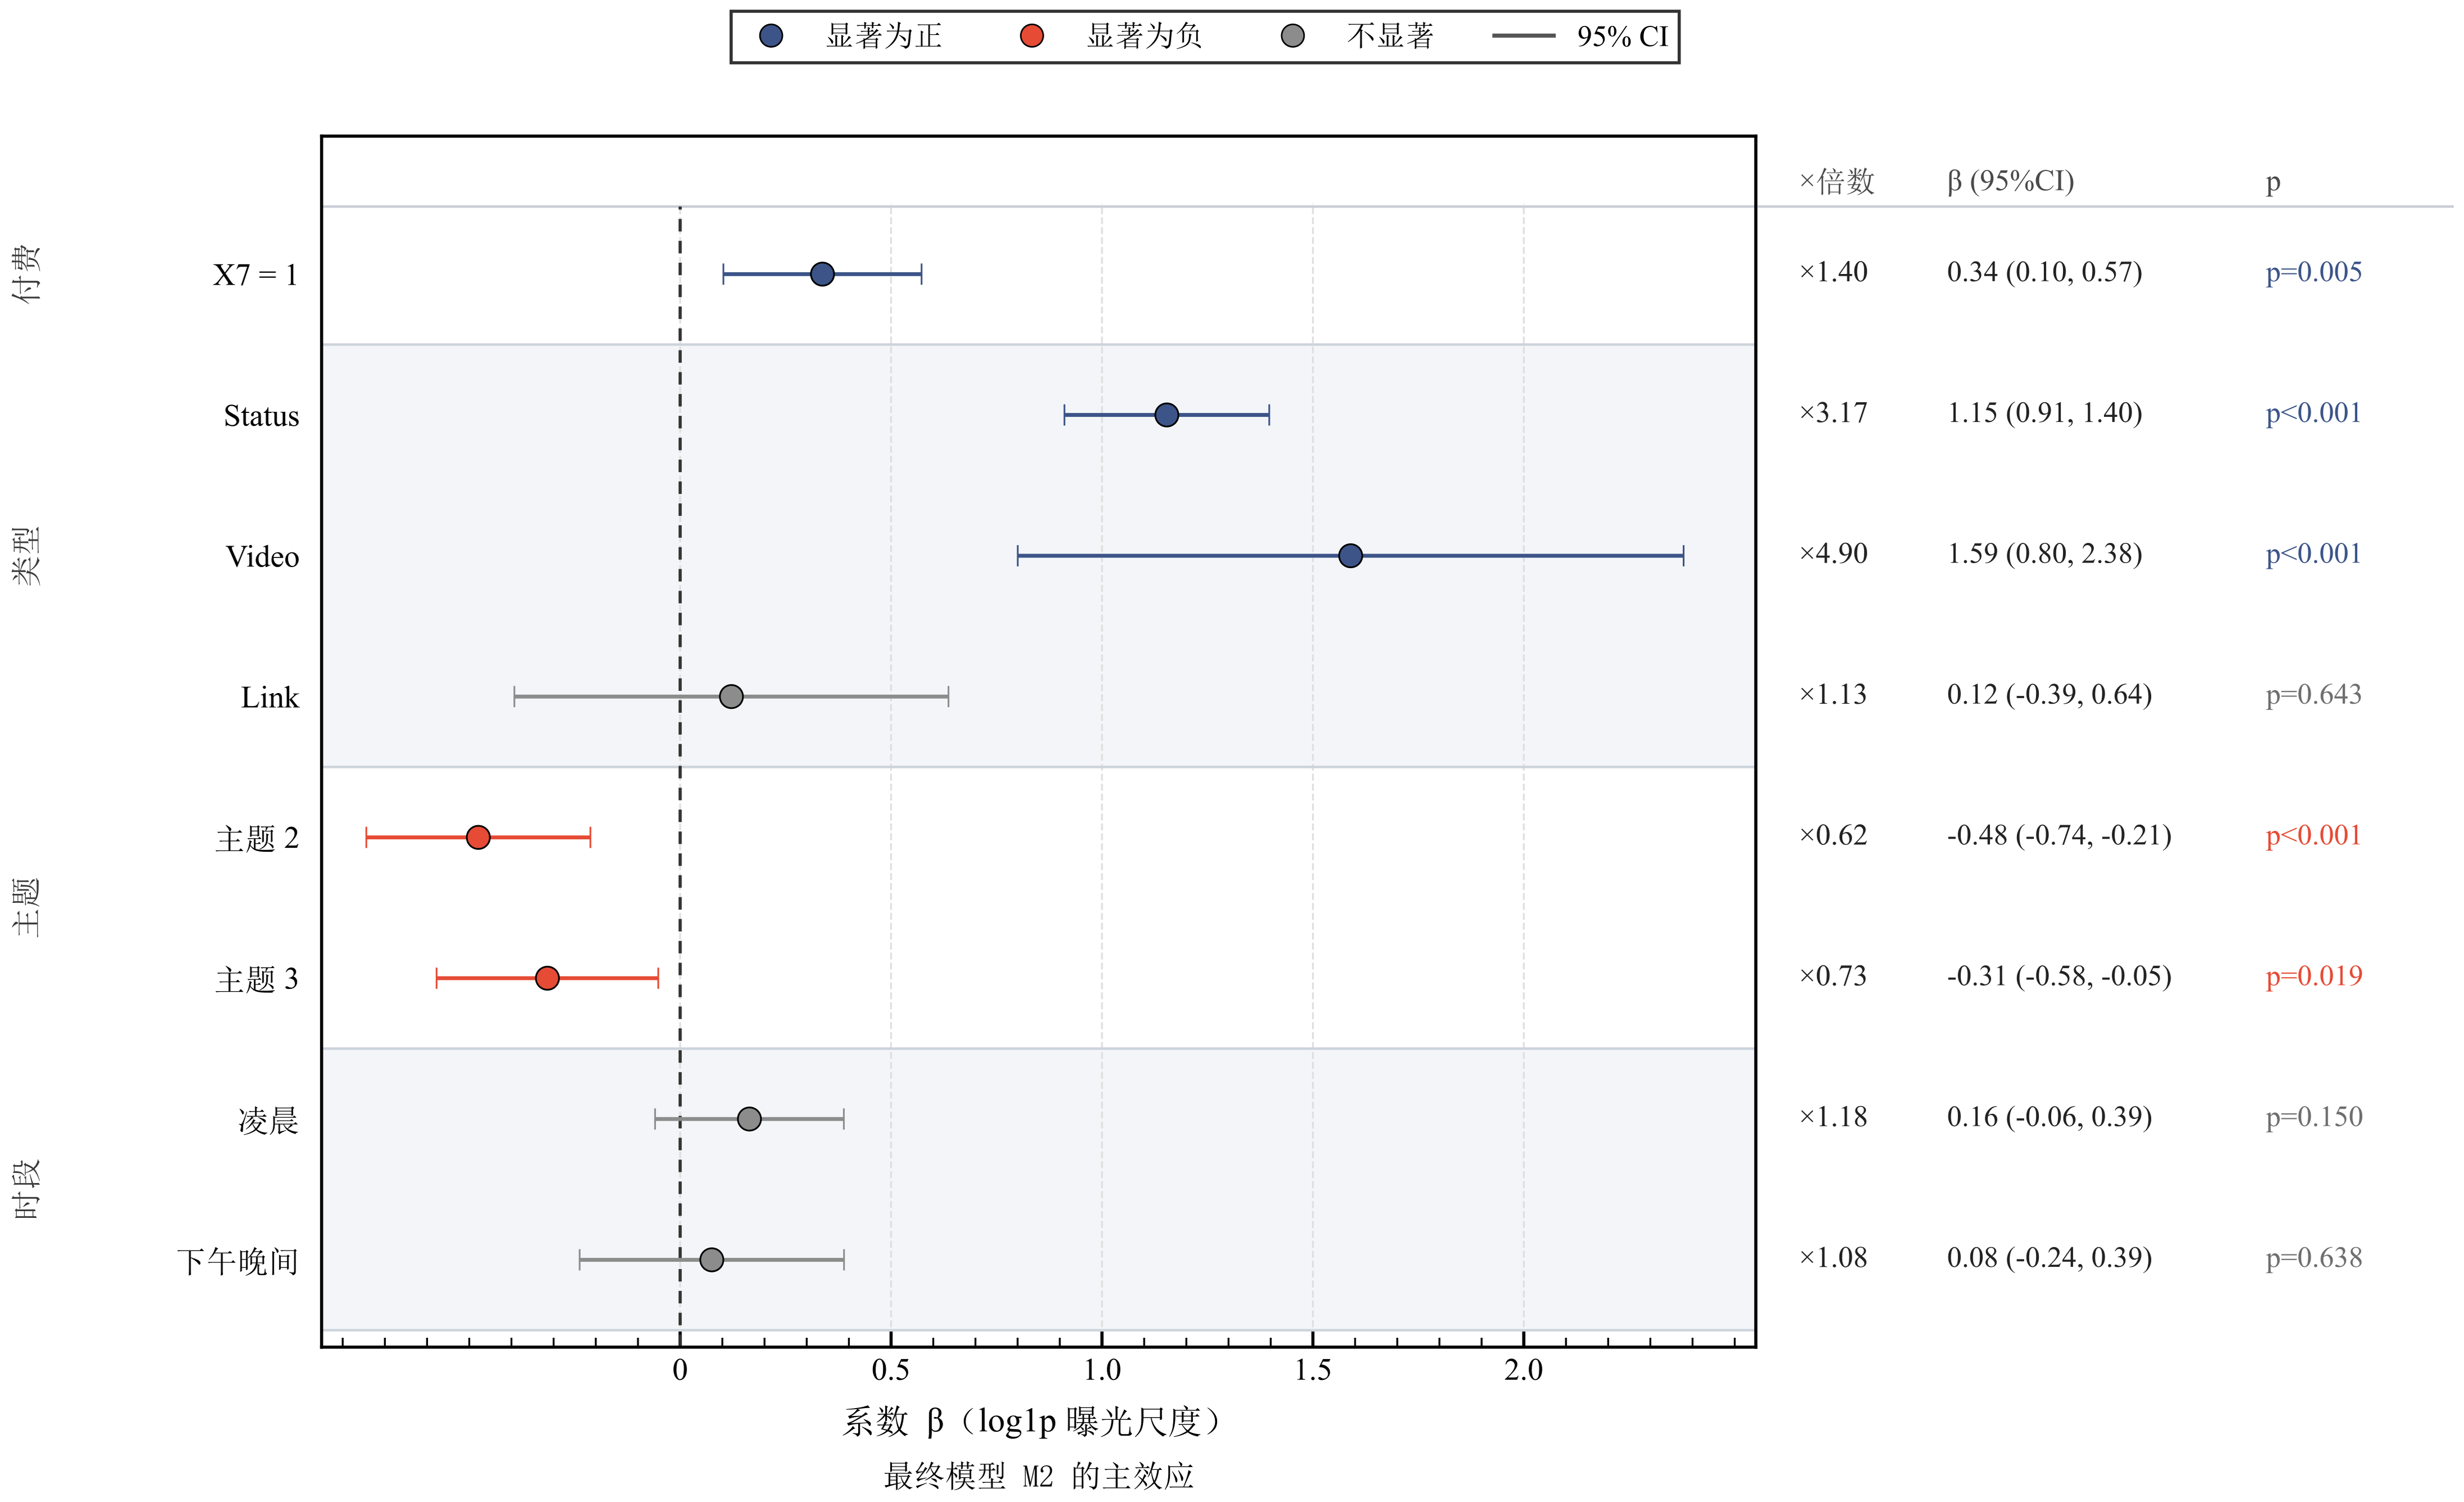
\includegraphics[width=0.76\textwidth]{../求解/问题三/结果/图6_最终模型系数森林图.png}
  \caption{最终模型的主效应系数与 95\% 置信区间}
  \label{fig:forest}
\end{figure}

\subsection{残差诊断与共线处理效果（对应 2.3.2-A、B）}

残差检验见表\ref{tab:resid}。最终模型 M2 的 Jarque--Bera 统计量 120.36、$p<0.001$，残差呈尖峰厚尾；Breusch--Pagan 统计量 54.74、$p=0.0005$，存在随拟合值增大的异方差；White 检验同样拒绝同方差（$p=0.030$），Ramsey RESET 未拒绝“线性形式正确”（$p=0.059$，处在临界）。这三项结果共同决定了推断口径：系数显著性使用 HC3 稳健标准误，系数解释限定在样本内的局部平均效应。图\ref{fig:resid}给出四联诊断：残差对拟合值呈水平带状但离散度随拟合值扩大；标准化残差的 Q--Q 图两端偏离 45° 线；尺度—位置图显示绝对残差随拟合值上升；Cook 距离有 30 个观测超过 $4/n$ 阈值，最大的三条分别为第 416、141、461 号帖子，其影响力均在可接受范围内。

\begin{figure}[t]
  \centering
  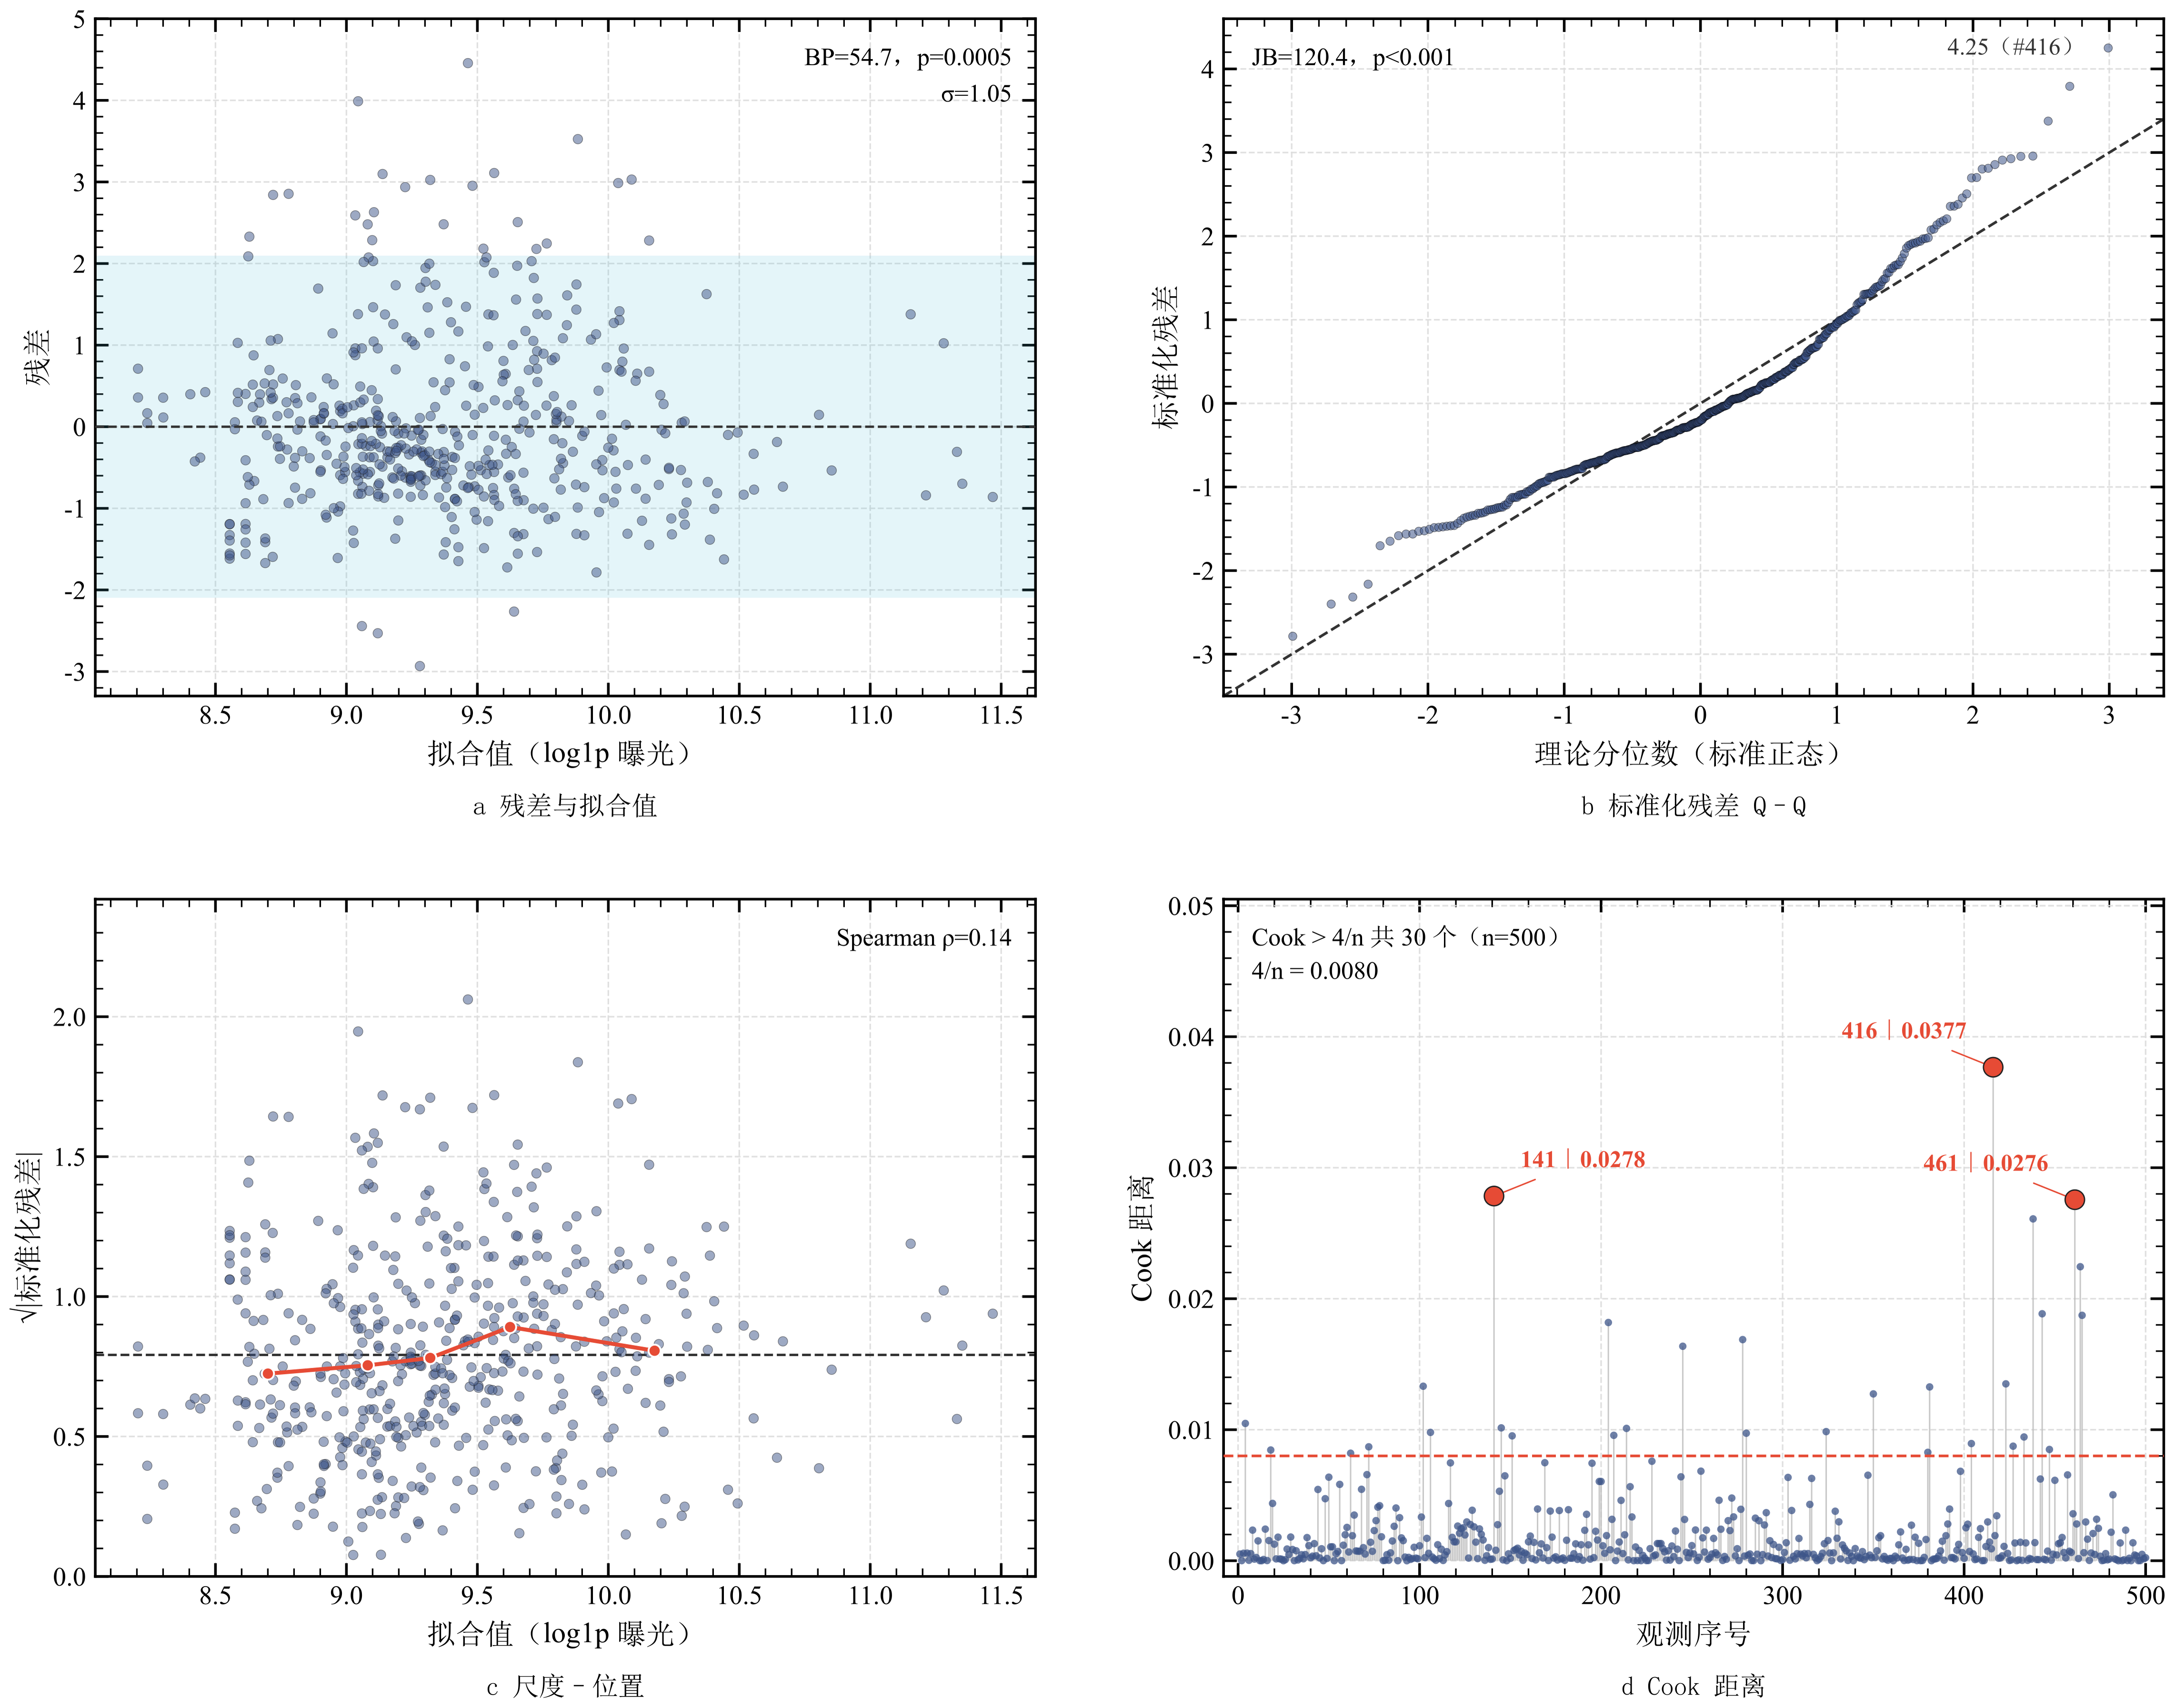
\includegraphics[width=0.58\textwidth]{../求解/问题三/结果/图8_残差诊断.png}
  \caption{最终模型的残差诊断：拟合、Q--Q、尺度—位置与 Cook 距离}
  \label{fig:resid}
\end{figure}

{\small
\begin{longtable}{>{\centering\arraybackslash}p{0.160\textwidth}>{\centering\arraybackslash}p{0.300\textwidth}>{\centering\arraybackslash}p{0.160\textwidth}>{\centering\arraybackslash}p{0.140\textwidth}>{\centering\arraybackslash}p{0.220\textwidth}}
  \caption{残差诊断检验结果}
  \label{tab:resid} \\
  \toprule
  模型 & 检验 & 统计量 & p值 & 判断 \\
  \midrule
  \endfirsthead
  \caption{残差诊断检验结果（续）} \\
  \toprule
  模型 & 检验 & 统计量 & p值 & 判断 \\
  \midrule
  \endhead
  \bottomrule
  \endfoot
  M1 全模型 & Jarque–Bera 正态性 & 119.0 & 0 & 残差非正态 \\
  M1 全模型 & Breusch–Pagan 异方差 & 56.5179 & 0.0005 & 存在异方差 \\
  M1 全模型 & White 异方差 & 283.3 & 0.0789 & 未检出/不可判定 \\
  M1 全模型 & Ramsey RESET（3 阶） & 2.867 & 0.0579 & 未检出设定误差 \\
  M1 全模型 & Durbin–Watson & 2.0513 & — & 接近 2，无强自相关（截面数据仅作参考） \\
  M1 全模型 & Cook 距离最大值 & 0.0492 & — & 无 Cook>1 的强影响点 \\
  M1 全模型 & 高杠杆点个数（h>2p/n） & 10 & — & 阈值 h>0.108 \\
  M2 最终模型 & Jarque–Bera 正态性 & 120.4 & 0 & 残差非正态 \\
  M2 最终模型 & Breusch–Pagan 异方差 & 54.7371 & 0.0005 & 存在异方差 \\
  M2 最终模型 & White 异方差 & 266.5 & 0.0301 & 存在异方差 \\
  M2 最终模型 & Ramsey RESET（3 阶） & 2.8451 & 0.0591 & 未检出设定误差 \\
  M2 最终模型 & Durbin–Watson & 2.0523 & — & 接近 2，无强自相关（截面数据仅作参考） \\
  M2 最终模型 & Cook 距离最大值 & 0.0377 & — & 无 Cook>1 的强影响点 \\
  M2 最终模型 & 高杠杆点个数（h>2p/n） & 10 & — & 阈值 h>0.104 \\
\end{longtable}
}




共线处理的直接效果见图\ref{fig:vif}。全模型 M1 中 $\log X_1$ 的方差膨胀因子为 124.9、月份哑变量组最大值为 143.0，远超 10 的严重共线阈值；剔除粉丝规模后，M2 的最大方差膨胀因子降至 3.23，全部解释变量落入可接受区间（$<5$）。哑铃图把每个变量的前后变化连在一起，除粉丝规模已不进入模型外，其余变量的方差膨胀因子几乎不变，说明共线只发生在粉丝规模与月份之间，与其他变量无关。

\begin{figure}[htbp]
  \centering
  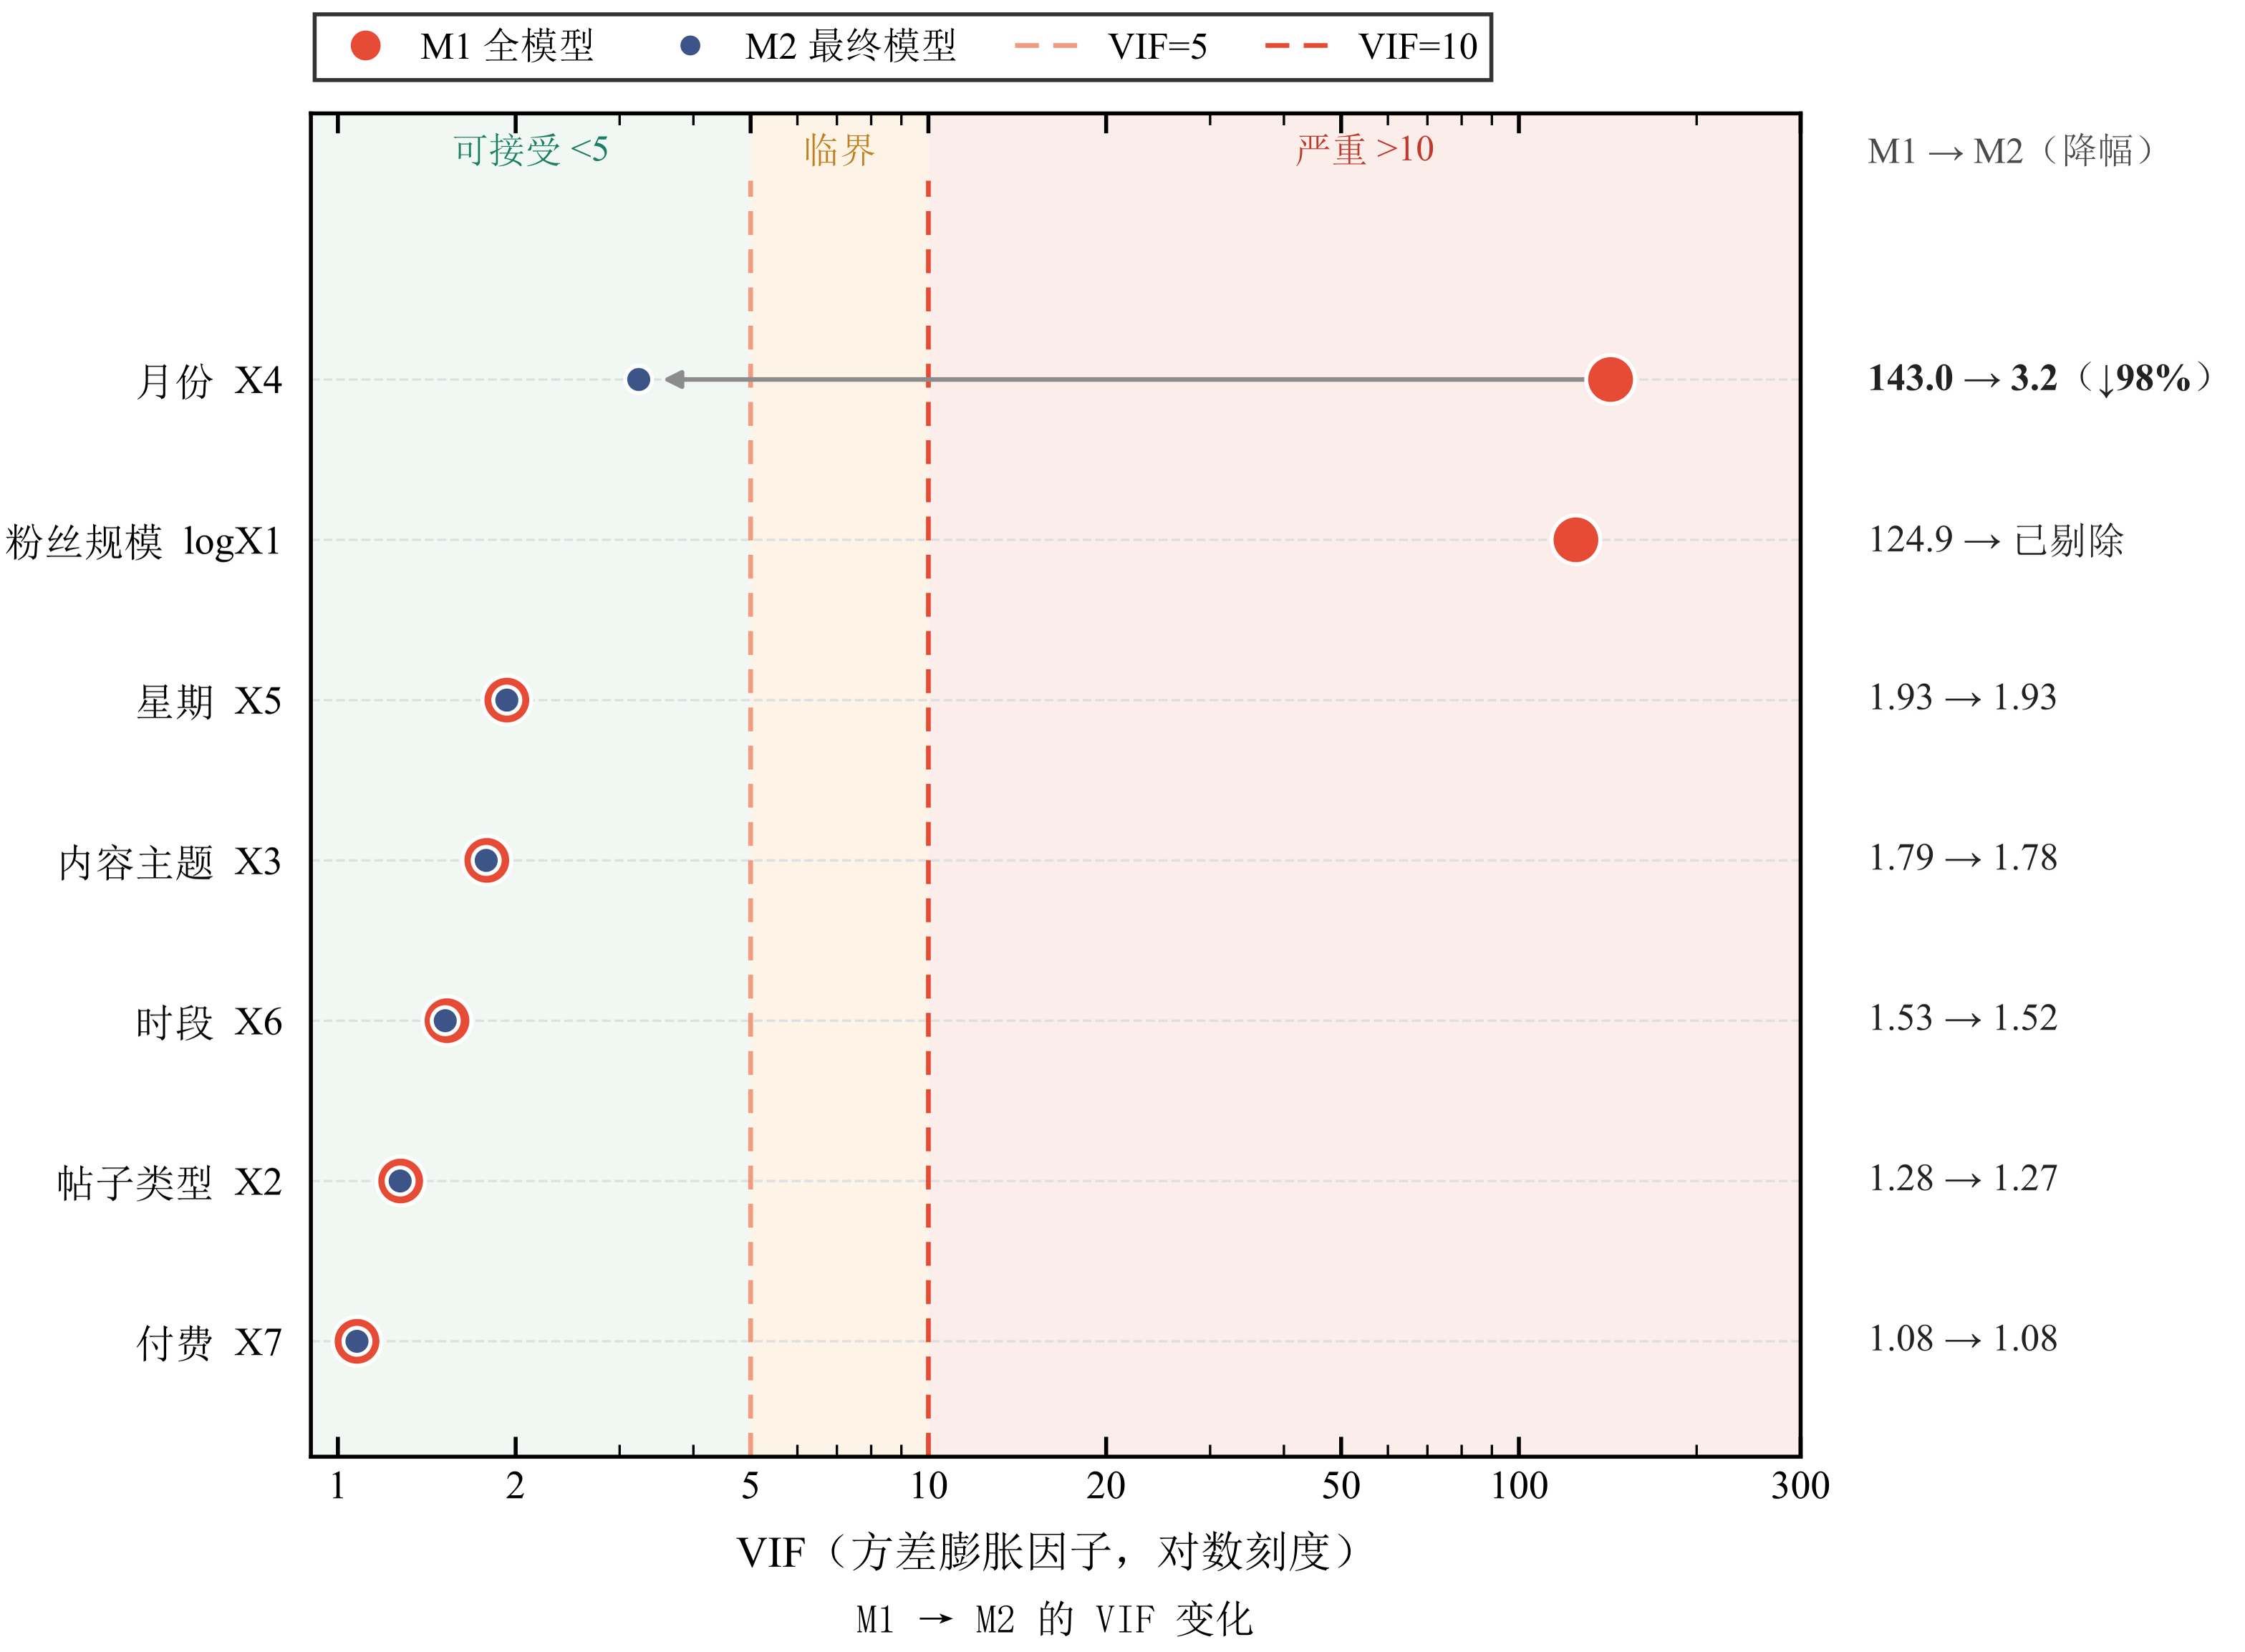
\includegraphics[width=0.58\textwidth]{../求解/问题三/结果/图7_共线性诊断.png}
  \caption{共线处理前后各方差膨胀因子的变化}
  \label{fig:vif}
\end{figure}

\subsection{预测能力（对应 2.3.2-D）}

图\ref{fig:cv}把五个候选的样本内 $R^2$ 与十折交叉验证 $R^2$ 用坡度图对照。所有模型都出现右倾——交叉验证表现低于样本内，这是参数估计用到全部样本的必然结果，但倾斜幅度不同：M1 从 0.207 降至 0.097，M2 从 0.207 降至 0.101，两者几乎重合；M3 与 M4 分别从 0.161 与 0.166 降至 0.094 与 0.097；M0 从 0 降至 $-0.021$。M2 的交叉验证 $R^2$ 最高、RMSE 最低，且比 M1 少一个参数，因此作为最终模型。样本外 $R^2$ 只有 0.10，说明模型适合判断变量方向与相对幅度，不适合逐条预测单帖曝光。

\begin{figure}[htbp]
  \centering
  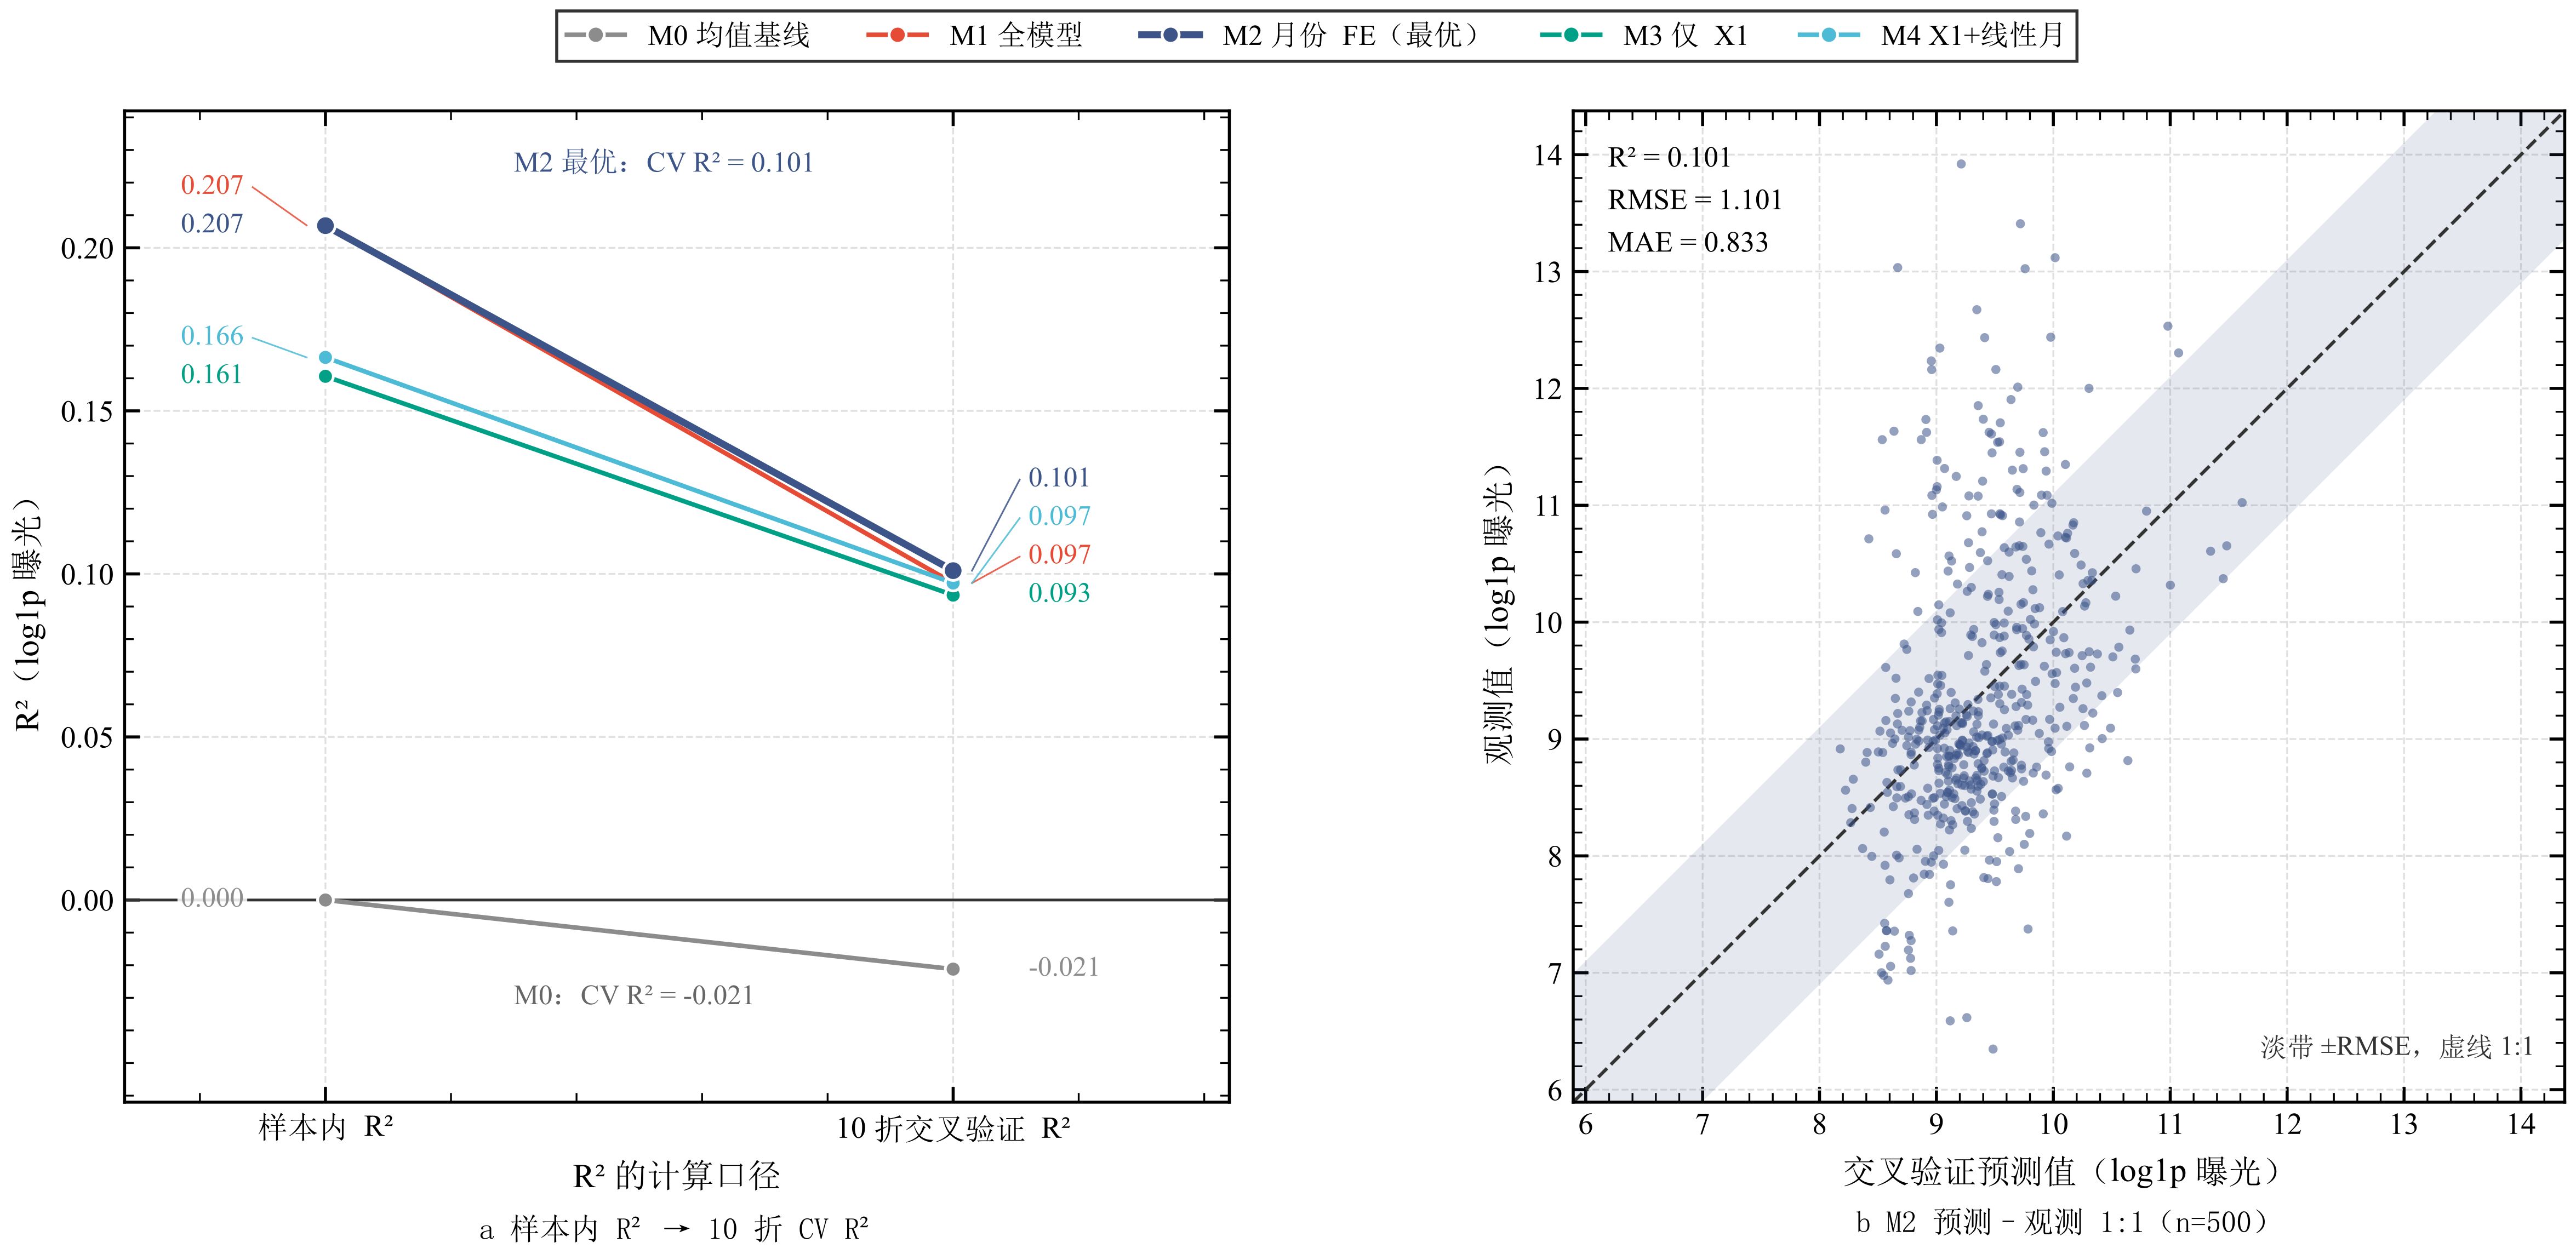
\includegraphics[width=0.76\textwidth]{../求解/问题三/结果/图9_预测能力验证.png}
  \caption{五个候选模型的样本内与交叉验证 $R^2$}
  \label{fig:cv}
\end{figure}

\subsection{方差贡献分解}

把七个变量组按 128 个子集做 Shapley 分解，结果见表\ref{tab:shap}：发帖类型贡献 0.0767（占可解释方差 37.1\%）、月份 0.0579（28.0\%）、付费 0.0244（11.8\%）、星期 0.0236（11.4\%）、内容主题 0.0142（6.9\%）、时段 0.0055（2.6\%）、粉丝规模 0.0046（2.2\%）。七个变量组合计解释 20.7\% 的曝光方差，剩余 79.3\% 属于个体差异与未观测因素。这一分解给出与回归系数一致的排序：发帖类型与月份是曝光差异的主要来源，付费与星期次之，粉丝规模在控制月份后几乎没有增量贡献。

\needspace{16\baselineskip}
{\small
\begin{longtable}{>{\centering\arraybackslash}p{0.240\textwidth}>{\centering\arraybackslash}p{0.120\textwidth}>{\centering\arraybackslash}p{0.200\textwidth}>{\centering\arraybackslash}p{0.220\textwidth}>{\centering\arraybackslash}p{0.200\textwidth}}
  \caption{七个变量组的 Shapley $R^2$ 分解}
  \label{tab:shap} \\
  \toprule
  变量组 & 自由度 & Shapley\_R² & 占已解释方差 & 占总方差 \\
  \midrule
  \endfirsthead
  \caption{七个变量组的 Shapley $R^2$ 分解（续）} \\
  \toprule
  变量组 & 自由度 & Shapley\_R² & 占已解释方差 & 占总方差 \\
  \midrule
  \endhead
  \bottomrule
  \endfoot
  发帖类型 X2 & 3 & 0.0767 & 0.3709 & 0.0767 \\
  内容主题 X3 & 2 & 0.0142 & 0.0688 & 0.0142 \\
  月份 X4 & 11 & 0.0579 & 0.2798 & 0.0579 \\
  星期 X5 & 6 & 0.0236 & 0.1142 & 0.0236 \\
  时段 X6 & 2 & 0.0055 & 0.0264 & 0.0055 \\
  付费 X7 & 1 & 0.0244 & 0.1179 & 0.0244 \\
  粉丝规模 logX1 & 1 & 0.0046 & 0.0220 & 0.0046 \\
  发帖决策合计（X2/X3/X5/X6/X7） & 13 & 0.1445 & 0.6982 & 0.1445 \\
  账号规模与时间合计（X1/X4） & 12 & 0.0624 & 0.3018 & 0.0624 \\
  未解释方差 & — & 0.7931 & — & 0.7931 \\
\end{longtable}
}


